\chapter{Introducción}
\label{cha:introduccion}



Este libro está diseñado con un público muy particular en mente, tal y como se establece en el título: estudiantes de ingeniería que deben escribir toda su tesis en este gran sistema de composición de textos que es \LaTeX{} (cuando lo leas en tu mente, que se escuche algo como \emph{leitec}, no como material de preservativos).

Por supuesto, al empezar a trabajar con \LaTeX{} hace años esos no eran los adjetivos que utilizaba para describir este sistema, y más bien lo definía como ``una herramienta tecnológica de tortura del siglo XX usada por la Inquisición Académica''.

Resulta que las imágenes no se insertaban al ser arrastradas al editor, y tampoco se quedaban donde yo les decía, ¿para qué servía el código entonces? Introducir caracteres en español era un horror, y los fragmentos de código que insertaba solo respetaban el alfabeto inglés, convirtiendo las letras acentuadas en símbolos horribles\footnote{Vale, no eran símbolos extraídos del \emph{Necronomicón}, pero me causaron pesadillas por mi ignorancia.}. Posiblemente, la mitad de mi tesis se fue en una pelea infructuosa en contra de \LaTeX.

Si tanta fue mi agonía, ¿por qué me empeñé tanto en usar \LaTeX{}  como sistema de composición de un documento tan extenso como lo fue mi tesis? Por una razón: era requisito, al menos en mi carrera (un requisito no compartido uniformemente en mi institución, lo que solo sirvió para incrementar mi frustración en aquellos ayeres).

Quizá esta es tu primera exposición a \LaTeX, y has comenzado de una manera similar a la mía: sabrá Dios qué es, sabrá Dios cómo se usa\footnote{Como este es un documento laico, esta es la única referencia a una deidad que verás aquí.}, pero un director de tesis anticuado desea que redactes en esta cosa compleja, que ni interfaz tiene, que parece más código que otra cosa, y que no sabes por qué tienes que utilizar si existe Word.

Lo bueno es que estás de suerte porque este libro lo escribí como respuesta a ``¿Qué hago si tengo que utilizar \LaTeX{} para escribir mi tesis y no sé dónde empezar?''
Mi objetivo es evitarte muchas de las frustraciones que yo sufrí durante la redacción de mi tesis mientras aprendía a utilizar \LaTeX{}. Pero he de advertirte: esta obra contiene algunas de mis vivencias como tesista y algunas opiniones personales, incluidas con el objetivo de hacer amena la lectura. Toma lo que te sirva, desecha lo que no.

Definido el tono del libro, comencemos con la teoría.



\section{¿Qué es?}
\label{sec:que_es}



Si no te preguntas qué es \LaTeX{}, haces bien, ¿para qué saber? Ah, cierto, requisitos que cumplir\footnote{Si estás aquí por gusto, eres de la inimaginable minoría. Igual será un placer ser tu guía.}. Comencemos definiendo lo que \emph{no es}. \LaTeX{} no es un sistema \emph{WYSIWYG} (lo que ves es lo que obtienes\footnote{Del inglés ``What You See Is What You Get''}) como lo es Microsoft Word, a pesar de que ya hay opciones que permiten generar un documento de \LaTeX{} en una interfaz algo similar. No obstante, sigue siendo mejor escribir el ``código'' que será el documento final.

Pero, ¿por qué? Con la existencia de procesadores de texto tan poderosos, con una interfaz amigable, ¿para qué molestarse en aprender a utilizar \LaTeX, que aparenta ser tan arcaico? ¿Por qué nadie se ha preocupado en hacer una interfaz para que \LaTeX{} sea tan \emph{WYSIWYG} como Word?

Esas respuestas solamente se puede obtener indagando en las características de \LaTeX{}, mismas que nos ayudarán a definir qué es.



\subsection{Contenido sobre formato}
\label{ssub:contenido_sobre_formato}



\LaTeX{} se centra en el contenido. Si sabes un poco de páginas web, podríamos decir que \LaTeX{} es el equivalente al HTML de una página en el sentido de que define la estructura de cómo se debe desplegar el documento. Extendiendo la analogía, el código HTML no se puede visualizar sin un navegador que lo interprete. De la misma forma, \LaTeX{} necesita al compilador para pasar de código a documento presentable.

Aún más, podríamos decir que el CSS, la parte de una página que hace que se vea bonita, equivale a configuraciones de \LaTeX{} en el preámbulo, mismas que nos permiten modificar la presentación del contenido sin cambiar nada, o casi nada, del código utilizado durante la redacción.

En otras palabras, al redactar en \LaTeX{} no nos preocuparemos por el formato, al menos no en primera instancia, y posiblemente ni en segunda, ni en tercera. Es decir, no es necesario pensar en cómo se ven los títulos, la numeración de páginas, si el texto va justificado, o qué fuente vamos a utilizar, mientras estemos en la fase de redacción.

Tanto así que este libro empieza de lleno con el contenido, con enfoque en lo que vas a escribir, explicando cómo hacer listas numeradas o sin numerar, cómo meter imágenes, tablas o código, pero no brinda detalles de cómo cambiar cuestiones de estilo. Porque, de nuevo, importa más el contenido que el formato.

Además, si vas a redactar una tesis para tu institución educativa, lo más probable es que ya tengas una plantilla la cual tienes que seguir, a pesar de que la consideres un crimen en contra de todo sentido de la estética. Requisitos son requisitos.

No puedo terminar esta sección sin enfatizar nuevamente: el formato no es el protagonista en \LaTeX{}, ocúpate de escribir. Al último trabajaremos con la apariencia.



\subsection{Instrucciones}
\label{ssub:instrucciones}



Aún no vemos cómo se ve el código de un documento realizado con \LaTeX, pero basta decir que se asemeja mucho a código de computadora, a cosas ininteligibles para seres mortales. Sí, suena a complicaciones innecesarias para realizar un documento que parece destinado a solo satisfacer el ego de unos cuantos.

No obstante, lo que distingue a \LaTeX{} es precisamente esta forma de trabajar, estas instrucciones que al final del día conforman el documento final, y que van mano a mano del punto anterior: el contenido va primero, antes que todo formato.

¿Y qué es una instrucción? Es una orden o comando que la computadora tomará para traducirla desde tu ``yo escribo contenido'' al producto final en PDF\footnote{Se puede realizar una conversión a otros formatos, pero eso escapa el alcance de este libro.} de ``computadora genera formato''. Podemos verlo en términos de la figura \ref{fig:esquema_latex}:

% Código obtenido de https://web.iit.edu/sites/web/files/departments/academic-affairs/graduate-academic-affairs/pdfs/figure-help1.pdf
\begin{figure}[ht!]
	\setlength{\unitlength}{3.5mm} % selección de unidad de medida.
\centering % La figura se centra
\begin{picture}(32, 5)  % ancho * alto
	% Las coordenadas del comando "put" son en base a la esquina inferior izquierda.
	\put(9,0.5){\framebox(14,4){Instrucciones en \LaTeX}}
	\put(1.5,2.5){\vector(1,0){7.5}}
	\put(23,2.5){\vector(1,0){7.5}}
	\put(1.5,3){Nuestro texto}
	\put(24,3) {PDF final}
\end{picture}
	\caption{Esquema de trabajo en \LaTeX.} % Leyenda de la figura.
	\label{fig:esquema_latex}
\end{figure}

Como ejemplo, para generar este libro solo pensé en este capítulo como ``Introducción''. Al momento de escribir, no sabía si sería ``Capítulo 1'', ``Capítulo I'', o solo diría ``1'', o si estaría numerado, siquiera.

No me preocupé de si estaría alineado a la derecha o a la izquierda, o el tamaño de la letra. Simplemente introduje el siguiente código (técnicamente, es más correcto decir ``la siguiente instrucción'' pero suena mejor de esta manera):

\begin{lstlisting}[style=latex]
\chapter{Introducción}
\end{lstlisting}

Y con eso me liberé de preocuparme por el formato. Sí, en algún momento el cómo regresó a perseguirme, pero no mientras estaba escribiendo e investigando.

De la misma forma, no deberás ocuparte del formato mientras estés en la fase de \st{generar resultados falsos y rellenar con mentiras para llegar a un m\'inimo de hojas} investigación, desarrollo, y documentación, sino hasta que tu asesor te diga que el contenido está bien aunque el formato no tanto.



\subsection{\TeX{} y \LaTeX{}}
\label{ssub:tex_latex}



En el punto anterior vimos que \LaTeX{} utiliza instrucciones para generar documentos. Pero, en realidad, \LaTeX{} no es otra cosa que \TeX{} con esteroides. ¿Qué significa ésto? ¿Acaso existen otras versiones? ¿Qué importa si es \LaTeX, \TeX, Lua\TeX, o sabrá que otra abominación con \TeX{} al final?

No es que importe mucho en sí la historia, pero un tío llamado Donald Knuth creó \TeX{} allá por 1978, con una licencia de código abierto. De ahí, otras personas empezaron a empalmar sus modificaciones y atajos, como más formas de estilizar texto, o para sus aplicaciones particulares de fórmulas, código, alfabetos, y más.

Entonces, \LaTeX{} viene a ser la forma más popular de \TeX{} que existe, con macros o instrucciones agregadas por muchísima gente a lo largo de ya más de cuarenta años.

Por tomar otra analogía de los chicos de sistemas, \LaTeX{} vendría a ser como Ubuntu, la versión de Linux más conocida, y \TeX{} algo así como Debian, el papá de los pollitos. Y todas las demás variantes, que encontrarás muchas, son distintos sabores de \TeX{} para aplicaciones particulares.

¿Y eso qué tiene que ver con nosotros? Bueno, es hora de colocar el último clavo sobre el ataúd de la definición de \LaTeX.



\subsection{Infinidad de paquetes}
\label{ssub:infinidad_de_paquetes}



Ahora que hemos hablado de las instrucciones, como |\chapter|, y sabemos que \LaTeX{} es una versión aumentada de \TeX{} gracias a contribuciones de muchas personas, podemos entender la definición de \LaTeX{} (según Wikipedia \cite{bib:wiki_latex}):


\begin{displayquote}
\LaTeX{} es un sistema de composición de textos que está formado mayoritariamente por órdenes construidas a partir de comandos de \TeX.
\end{displayquote}

\noindent Con lo que hemos visto podemos construirnos una definición de mayor utilidad:

\begin{displayquote}
\LaTeX{} es una herramienta quimera, nacida de \TeX, que ha ido creciendo gracias a contribuciones de personas a lo largo de cuarenta años, cuyo objetivo es que podamos crear un documento que luce espectacular, enfocándonos mayormente en el contenido.
\end{displayquote}

Por supuesto, ese objetivo muchas veces se pierde entre tantas instrucciones y sabores. ¡Más de cuarenta años de personas agregando paquetes sin orden ni concierto! Sin una guía, es difícil comprender cómo podemos lograr nuestro objetivo de la manera más sencilla, sin que una instrucción afecte a otra.

Además, esta misma infinidad de paquetes hace que un editor \emph{WYSIWYG} sea poco factible, ¿cómo hacerlo si hay miles de paquetes que pueden modificar el comportamiento de las instrucciones? Sí, claro, el entorno \texttt{itemize} es una lista, por ejemplo, ¿pero cómo debe verse? Volvemos al mismo punto: importa más el hecho de que sea una lista, independientemente del cómo se ve. Por lo tanto, no tiene mucho sentido ver el resultado aproximado en tiempo real (como en Word) sino que podemos esperar para ver el resultado visual tras la fase de compilación.

¿Compila-qué? No te preocupes, ya llegaremos a ello en este mismo capítulo. Por lo pronto, ya tenemos una definición de \LaTeX{} y sabemos más o menos para qué nos sirve. Es tiempo de realizar un primer ejemplo en una plataforma en línea.



\section{Overleaf}
\label{sec:overleaf}



En mis tiempos (\textbf{tose, tose}) no existía una plataforma en línea en la cual realizar un documento en \LaTeX. Ni siquiera era universal el Javascript, mucho menos se podía concebir un equipo que compilara en tiempo real y permitiera generar un PDF al vuelo de varios archivos de código.

Dejando de lado la nostalgia de un viejo, el punto es que existe una plataforma gratuita en línea que permite escribir documentos complejos de \LaTeX{}, sin problemas ni peros (bueno, si quieres colaborar con alguien o compilar desde Dropbox o GitHub sí hay costo, pero estamos empezando y no haremos nada así a lo largo de este libro). Dicha plataforma es \href{https://www.overleaf.com/}{Overleaf}\footnote{Por si ves esto impreso, el sitio es \href{https://www.overleaf.com/}{https://www.overleaf.com/}}, cuya página principal luce similar a la figura \ref{fig:overleaf_home}.

\begin{figure}[ht!]
	\centering
	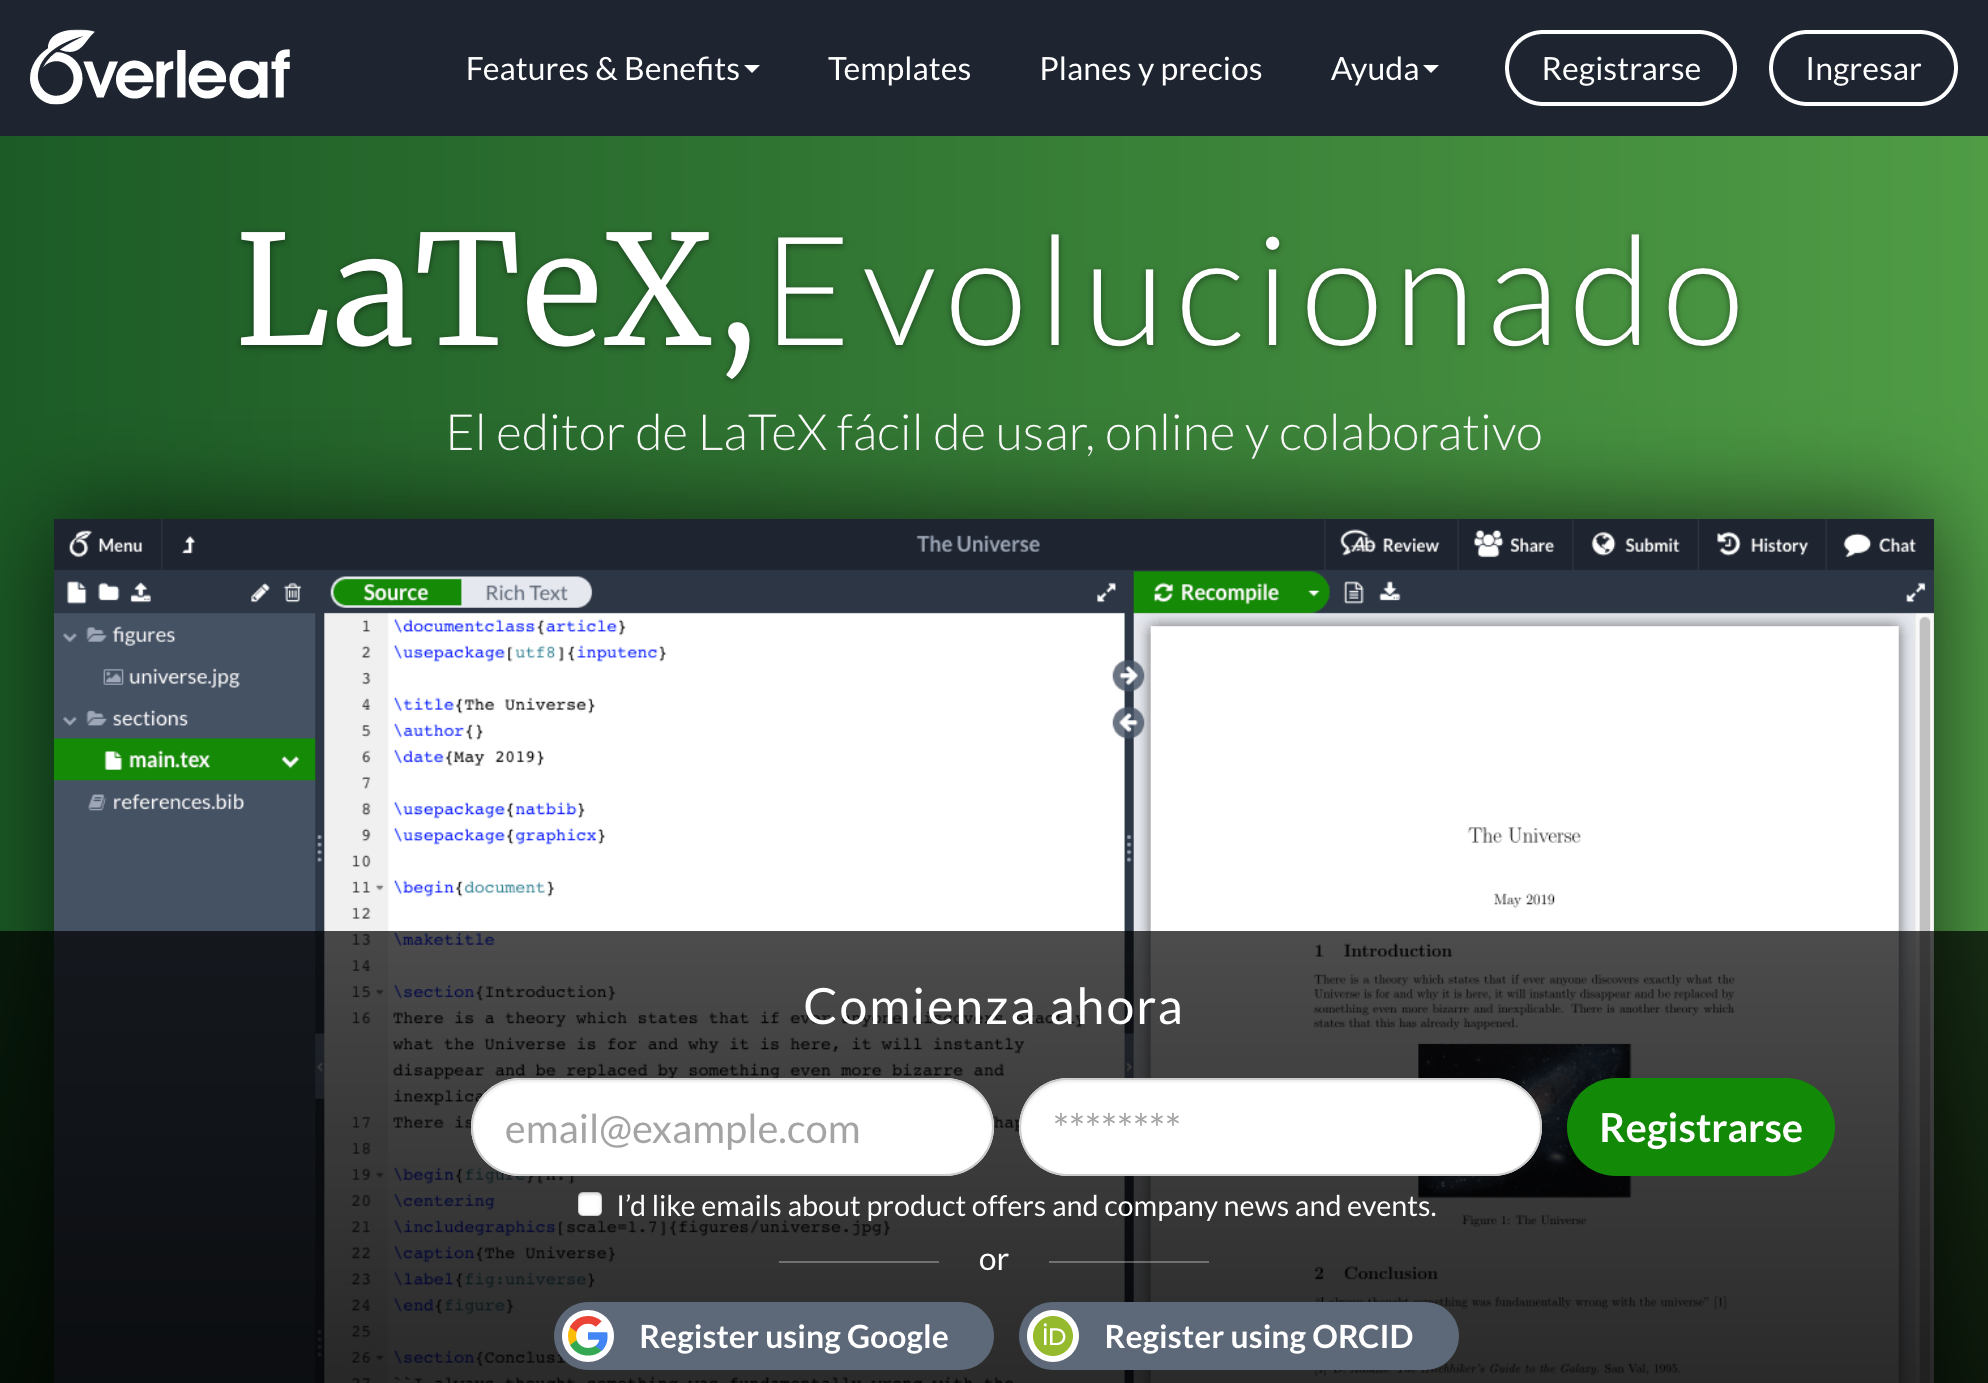
\includegraphics[width=\linewidth]{img/overleaf_300ppi.png}
	\caption{Página principal de Overleaf.}
	\label{fig:overleaf_home}
\end{figure}

En la figura \ref{fig:overleaf_home} se muestra el formulario de registro, el cual solo pide correo electrónico y contraseña, aunque también te puedes registrar mediante tu cuenta de Google. Una vez estés registrado, podemos empezar a crear el documento de prueba.



\section{Un primer documento}
\label{sec:un_primer_documento}



Dado que un documento de \LaTeX{} puede estar compuesto por muchos archivos, como después veremos, lo primero que hay que hacer es crear un proyecto (alias sofisticado de ``directorio'') en Overleaf, con \opcionMenu{Nuevo proyecto $\rightarrow$ Proyecto vacío}, como muestra la figura \ref{fig:overleaf_nuevo_proyecto_300ppi}. Aunque podemos crear proyectos a partir de ejemplos o de plantillas, empezaremos desde cero.

\begin{figure}[ht!]
	\centering
	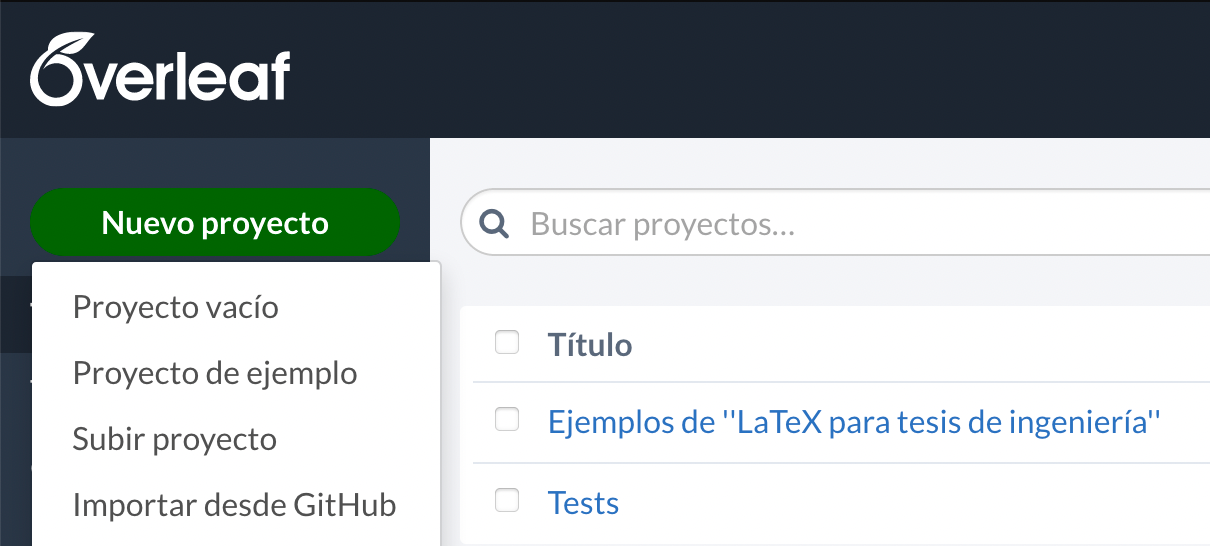
\includegraphics[scale=1]{img/overleaf_nuevo_proyecto_300ppi.png}
	\caption{Creando un nuevo proyecto en Overleaf.}
	\label{fig:overleaf_nuevo_proyecto_300ppi}
\end{figure}

Al dar clic en la opción \opcionMenu{Proyecto vacío} surgirá una pantalla modal, como la figura \ref{fig:overleaf_nombre_proyecto}, que preguntará por el nombre del proyecto. En mi caso, colocaré el nombre de \emph{Ejemplos de \textquotedbl{}LaTeX para tesis de ingeniería\textquotedbl{}}.

\begin{figure}[ht!]
	\centering
	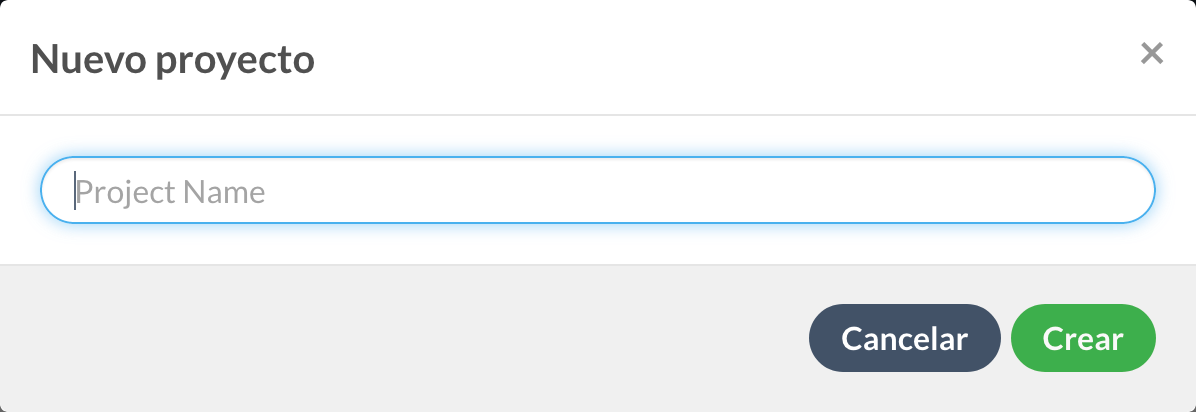
\includegraphics[width=112mm]{img/overleaf_nombre_proyecto_300ppi.png}
	\caption{Overleaf preguntando el nombre del nuevo proyecto.}
	\label{fig:overleaf_nombre_proyecto}
\end{figure}

Si todo sale bien, se desplegará una pantalla con información similar a lo que se muestra en la figura \ref{fig:overleaf_mi_primer_documento}, solo con un tamaño de fuente más pequeño. Obviamente el nombre del proyecto para ti será diferente (espero), así como el autor asignado de manera predeterminada. No obstante, en la columna izquierda debes tener un archivo llamado \texttt{main.tex}, en la columna central el contenido de dicho archivo, mientras que el lado derecho muestra el resultado en PDF con el nombre de tu proyecto, tu nombre como autor, y la fecha.

\begin{figure}[ht!]
	\centering
	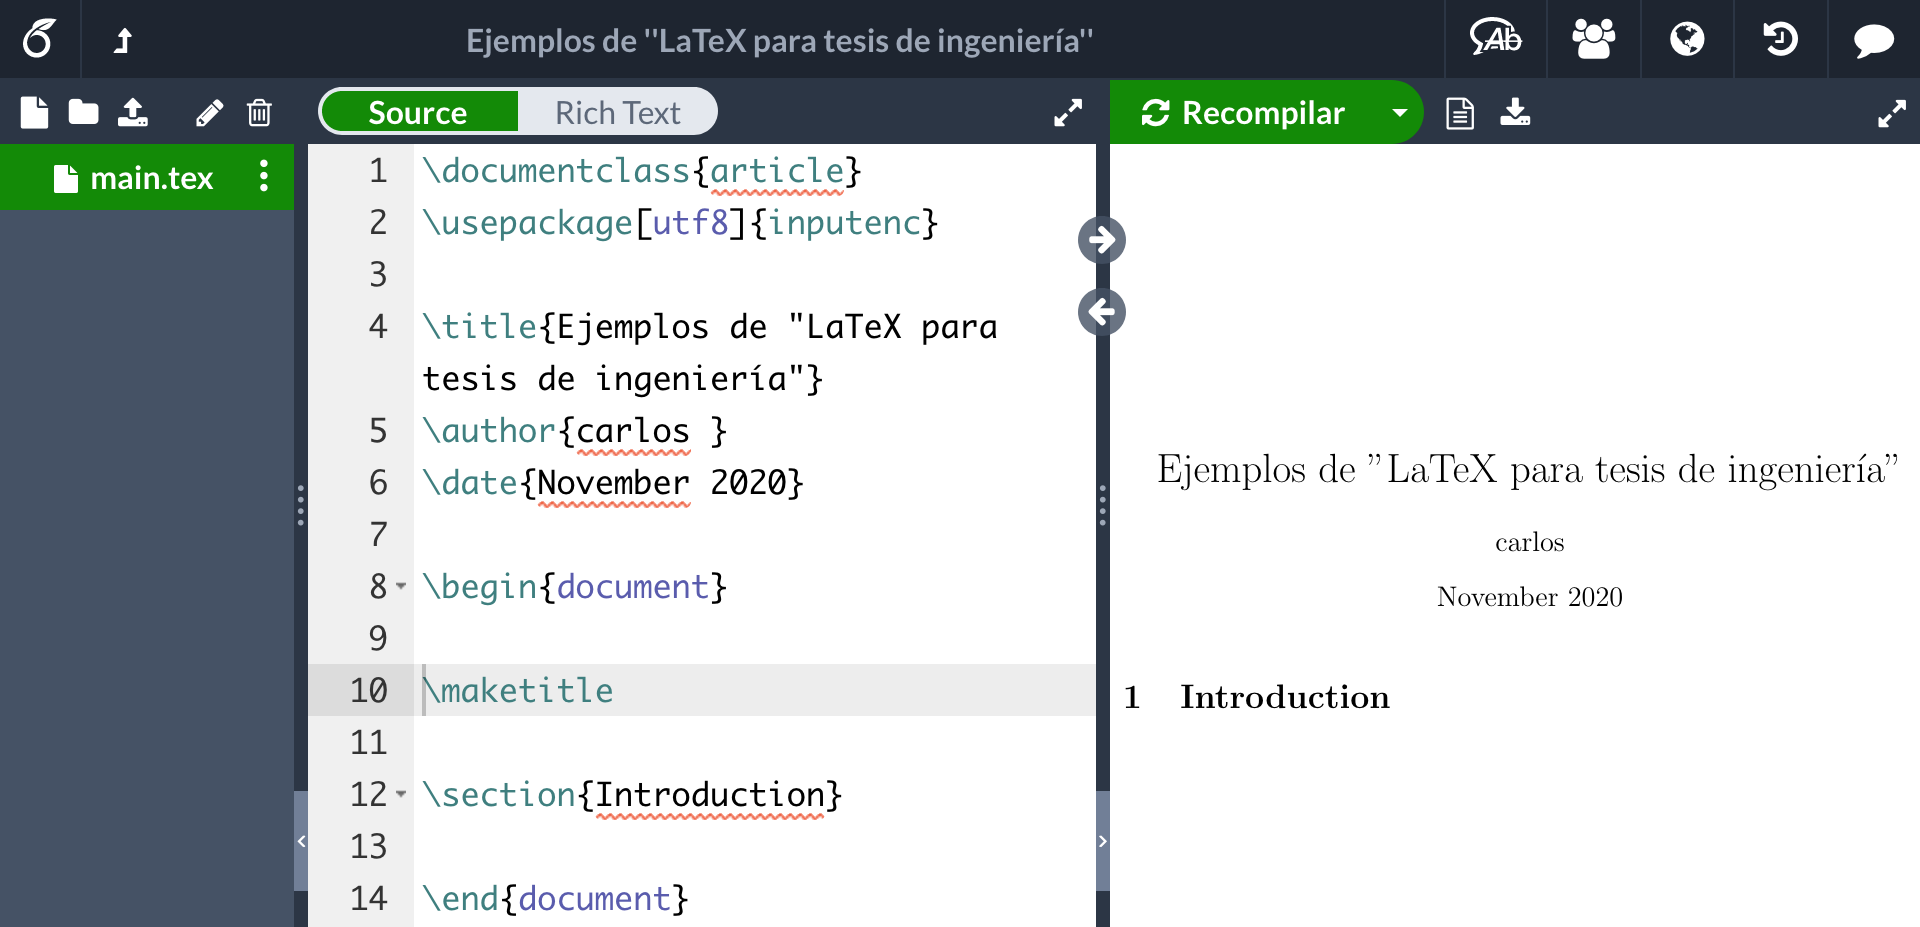
\includegraphics[width=\linewidth]{img/overleaf_mi_primer_documento_300ppi.png}
	\caption{Primer ejemplo en Overleaf.}
	\label{fig:overleaf_mi_primer_documento}
\end{figure}

Para empezar a comprender cómo funciona \LaTeX, revisemos el código del listado \ref{lst:mi_primer_documento}. En sí, lo que se puede deducir del PDF generado (lado derecho de la figura \ref{fig:overleaf_mi_primer_documento}) es que las líneas 4, 5, y 6 tienen un reflejo directo en el resultado final: se muestra el título del documento, el autor, y la fecha. También la línea 12 aparece en el documento, aunque el texto ``Introduction'' está precedido por un número.

¿Cómo es que esas cuatro líneas aparecen, una tras otra, pero en el código son separadas por la línea 8 y 10? ¿Y de dónde sale ese número asignado al texto en negritas de ``Introduction''? Y, claro, ¿por qué aparecen las comillas de cierre tanto al inicio como al final en nuestro título?

\lstinputlisting[label=lst:mi_primer_documento,numbers=left,style=latex,caption=Mi primer documento en \LaTeX.]{ejemplos/mi_primer_documento.tex}



\subsection{La instrucción \ttlatex{maketitle}}
\label{sub:la_instruccion_maketitle}



Empezaremos a responder las preguntas de manera empírica, eliminando la línea 10 del listado \ref{lst:mi_primer_documento}, que corresponde a la instrucción |\maketitle|. Se presiona el botón de \opcionMenu{Recompilar} y se observa el nuevo resultado, tal como muestra la figura \ref{fig:overleaf_sin_maketitle}.

\begin{figure}[ht!]
	\centering
	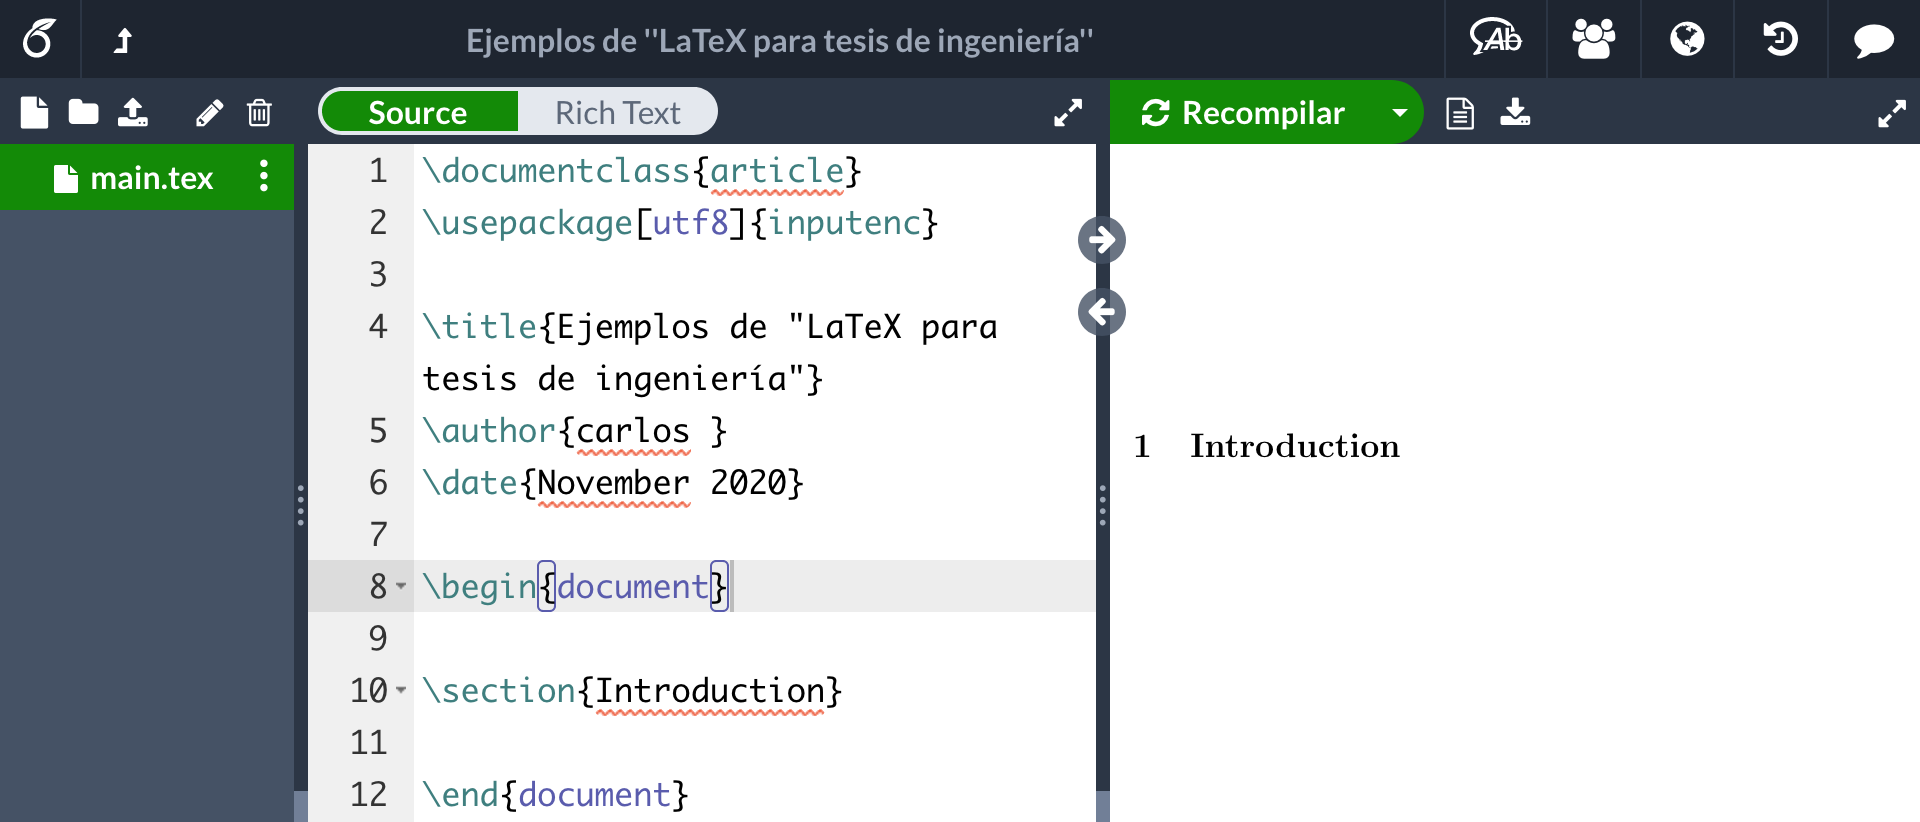
\includegraphics[width=\linewidth]{img/overleaf_sin_maketitle_300ppi.png}
	\caption{Primer ejemplo en Overleaf, sin \texttt{\textbackslash{}maketitle}.}
	\label{fig:overleaf_sin_maketitle}
\end{figure}

Dado que al eliminar la instrucción |\maketitle| ya no podemos ver en el PDF ni el título, ni el autor, ni la fecha, podemos asumir que esa instrucción se encargaba de mostrar esos tres datos centrados en el documento.

Y, basados en la misma información, podemos deducir que las instrucciones |\title|, |\author|, y |\date| son instrucciones para almacenar valores (ya que no imprimen en el documento), algo así como variables de \LaTeX, que la instrucción |\maketitle| puede leer e imprimir.

¿Importa cómo? No, solamente que lo hace. Debemos recordar que no tenemos motivos para preocuparnos por el formato o funcionalidad mientras se presente la información correcta en el documento.

Ya que sabemos los efectos de eliminar |\maketitle|, regresamos la línea a donde pertenece antes de continuar.



\subsection{La instrucción \texttt{\textbackslash{}section}}
\label{sub:la_instruccion_section}



La línea 12, |\section{Introduction}|, imprime ``Introduction'' precedido por un uno. Por ello, podemos asumir que \LaTeX, de alguna manera, enumerará consecutivamente las secciones. Haremos dos cosas para probar esta teoría:
\begin{enumerate}
	\item Cambiar el texto de ``Introduction'' a ``Introducción''.
	\item Crear una nueva sección llamada ``Esta sección debería llevar el número dos...''
\end{enumerate}

\begin{figure}[ht!]
	\centering
	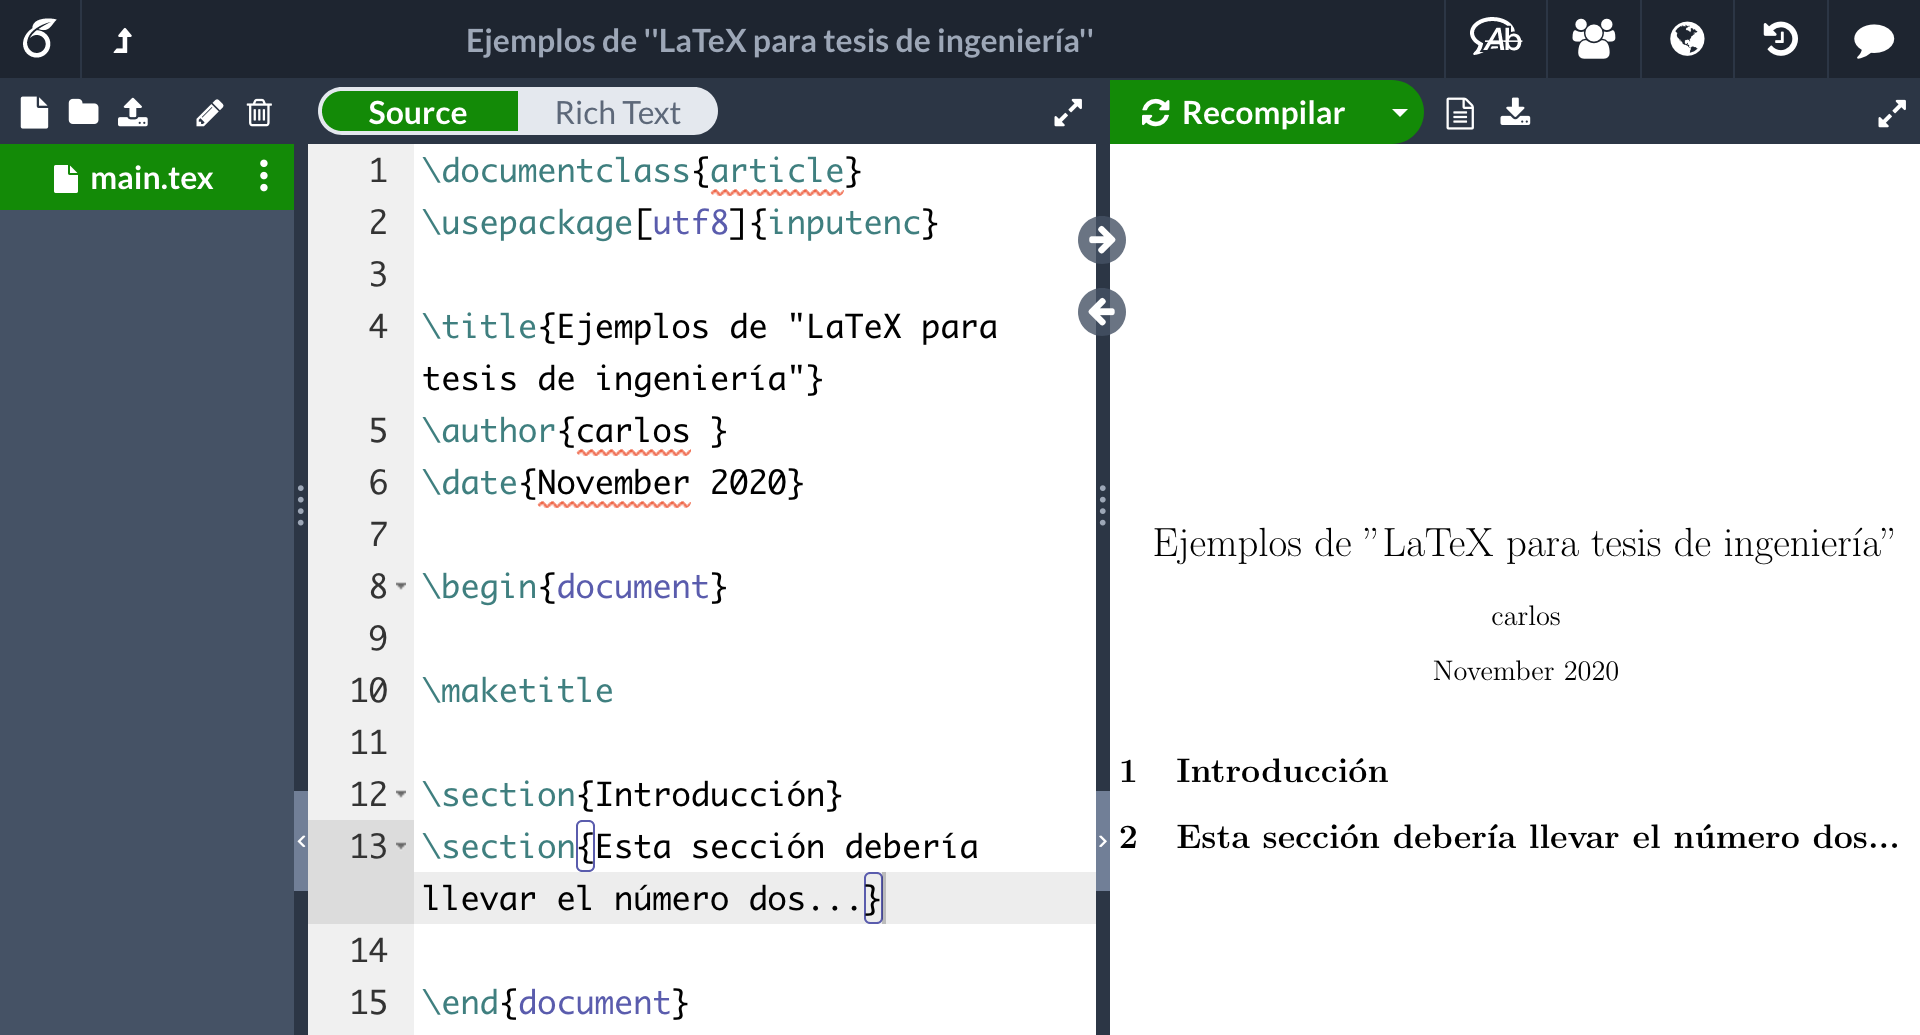
\includegraphics[width=\linewidth]{img/overleaf_seccion_dos_300ppi.png}
	\caption{Primer ejemplo en Overleaf, con una sección nueva.}
	\label{fig:overleaf_seccion_dos}
\end{figure}

La figura \ref{fig:overleaf_seccion_dos} refleja los cambios (tras volver a presionar el botón \opcionMenu{Recompilar}), y confirma las sospechas: \LaTeX{} agregará un consecutivo a cada sección, de manera automática, sin nuestra intervención (de nuevo, así nos preocupamos por la estructura del documento, no del cómo se ve). La líneas de código editadas fueron:

\begin{lstlisting}[style=latex]
\section{Introducción}
\section{Esta sección debería llevar el número dos...}
\end{lstlisting}



\subsection{Inicio y final de documento}
\label{sub:inicio_y_final_de_documento}



Siguiendo con el listado \ref{lst:mi_primer_documento}, las líneas 8 y 14 marcan el inicio y final del documento. ¿Esto qué quiere decir? Que todo lo que \emph{se ve} en el documento va entre estas dos instrucciones, por lo que si intentamos ejecutar el |\maketitle| antes de estas instrucciones, posiblemente se genere un error (y sí, la figura \ref{fig:overleaf_error_fuera_de_document} muestra el error que ocurre tras \opcionMenu{Recompilar}).

\begin{figure}[ht!]
	\centering
	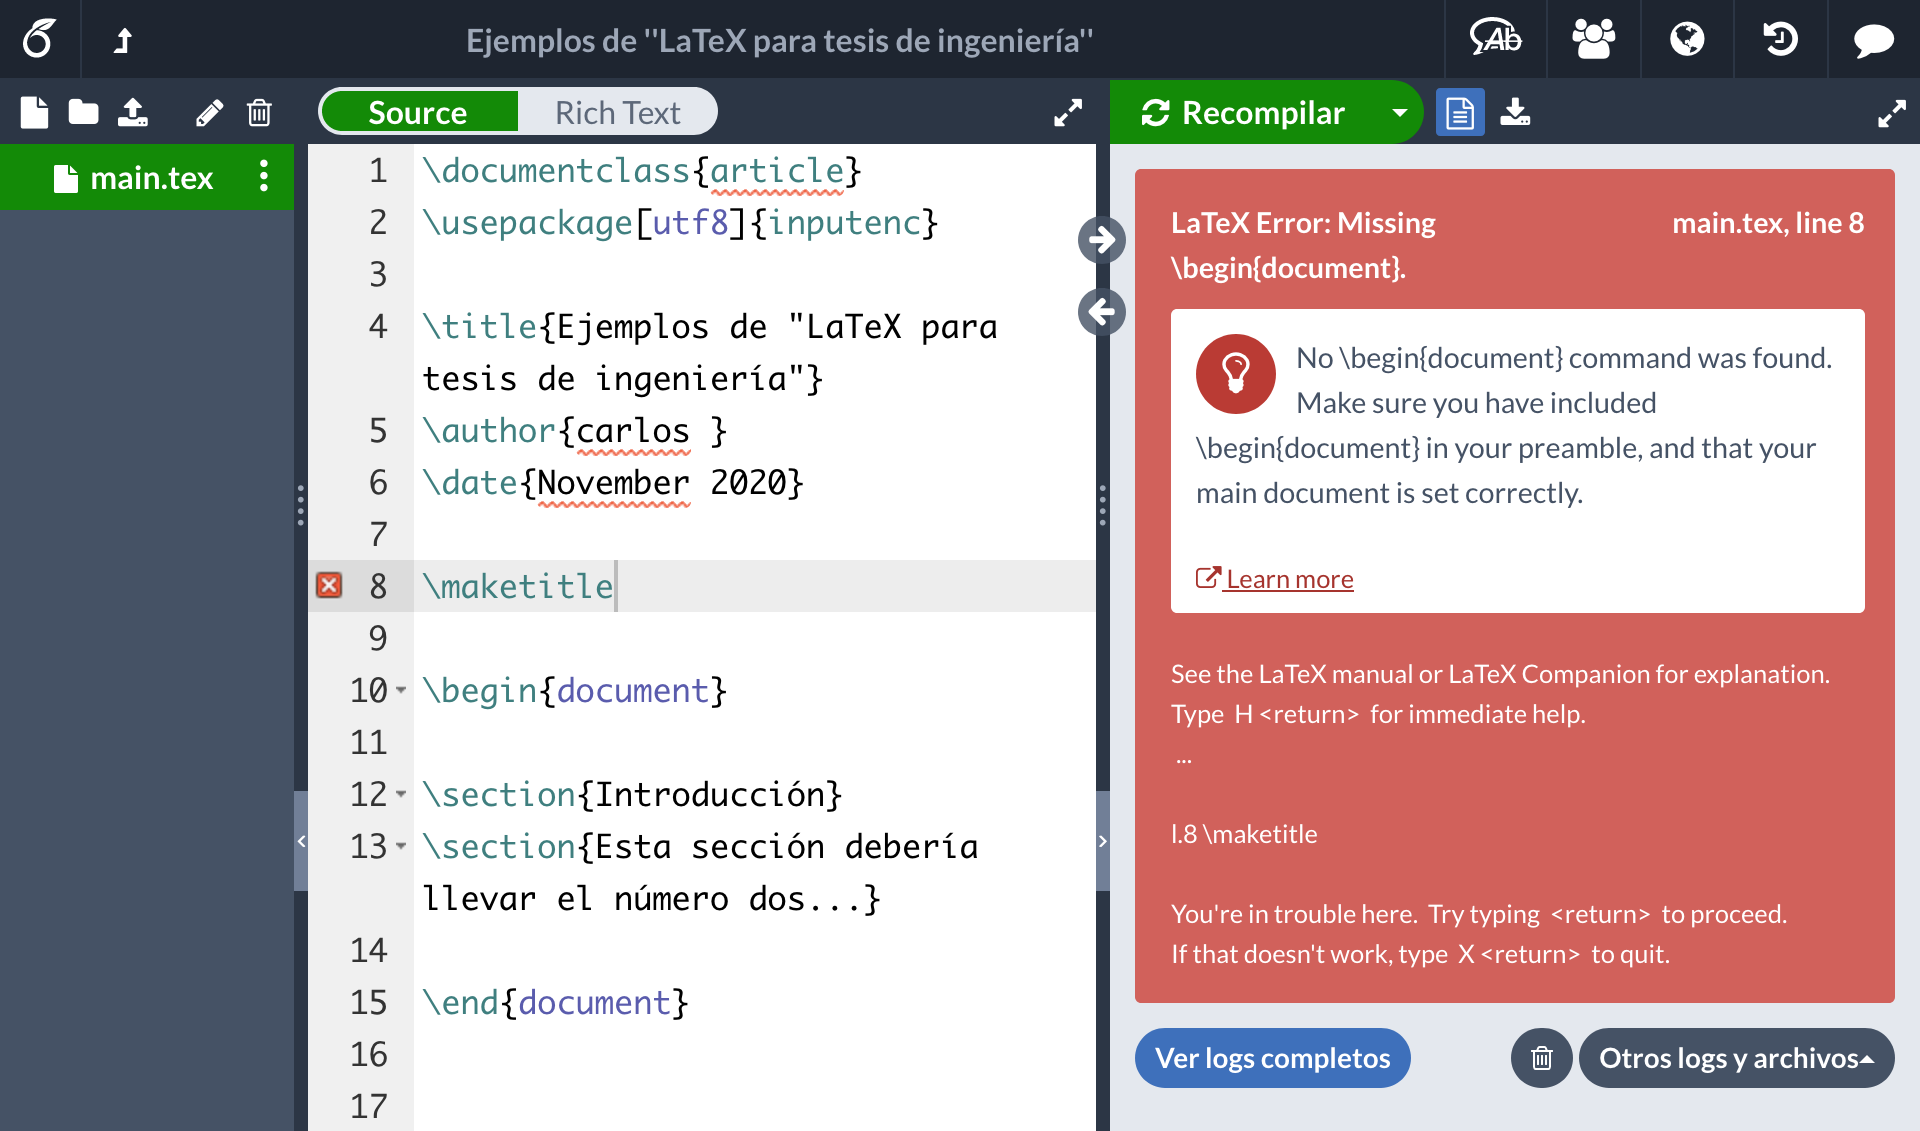
\includegraphics[width=\linewidth]{img/overleaf_error_fuera_de_document_300ppi.png}
	\caption{Primer ejemplo en Overleaf, con error fuera del \texttt{\textbackslash{}begin\{document\}}.}
	\label{fig:overleaf_error_fuera_de_document}
\end{figure}

De nuevo, no es nuestra intención conocer el cómo \LaTeX{} hace lo que hace, pero si algo va destinado a imprimirse o verse en pantalla, va entre |\begin{document}| y |\end{document}|. ¿Qué es lo que va fuera? Como en nuestro ejemplo, la declaración de ``variables'' como el autor, el título, y la fecha. También, la inclusión de paquetes que extienden las capacidades de \LaTeX{}.

En este primer documento ya se incluye el paquete \texttt{inputenc}.



\subsection{Texto en español (el paquete \texttt{\textbackslash{}inputenc})}
\label{sub:texto_en_espanol}



La instrucción |\usepackage| permite usar los paquetes que otra persona creó. Es decir, permite usar las instrucciones que alguien más ya hizo y decidió hacer públicas. Pero, en un ejemplo tan sencillo, ¿para qué necesitamos un cargar un paquete?

Cuando Donald Knuth creó \TeX{}, lo más probable es que pensara en sí mismo, sus fines, y su idioma (el inglés). Naturalmente, los acentos y las ``ñ'' no le pasaban por la mente, por lo que no son soportados de manera nativa. Para poder insertar los caracteres propios del idioma español, sin que estos sean convertidos a símbolos raros, se agrega el paquete \texttt{inputenc}, que permite definir en qué idioma estamos escribiendo (lo formal es decir algo como ``define la codificación de los caracteres de entrada'', pero se entiende menos).

Y una codificación\footnote{En inglés, \emph{encoding}.} muy utilizada, y que contiene los caracteres del español, es la UTF-8. No entraremos en detalles técnicos de representación, solo diremos que sin el paquete \texttt{inputenc} con la codificación \texttt{utf8} no se ven los caracteres en español de manera adecuada.

Como dato meramente informativo: este paquete no se incluye solamente porque tu Overleaf se haya configurado en español. El código ASCII quedó atrás hace mucho tiempo, siendo el UTF-8 el nuevo estándar de codificación. Así que, aunque tu documento solo utilice caracteres del idioma inglés, se recomienda utilizar el paquete UTF-8 (razón por la que Overleaf lo carga de manera predeterminada).



\subsection{Clase del documento}
\label{sub:clase_del_documento}



Dejamos la primera línea para el final, donde se define la clase del documento. Hay varias clases de documento, y muchas más si contamos las plantillas como el \href{https://www.latextemplates.com/template/tufte-style-book}{libro Tufte}, pero a lo largo de este libro utilizaremos artículos (clase \texttt{article}) y libros (clase \texttt{book}).

Los artículos serán utilizados para hacer las demostraciones cortas, como el listado \ref{lst:mi_primer_documento}, y el libro es la base de este documento, del cual tienes todo el código fuente a tu disposición.

Aunque existen muchas diferencias entre ambas clases, una de las principales es la estructura, o la forma en la que se subdivide, como se muestra en las siguientes listas:

\begin{multicols}{2}
Libro
\begin{itemize}
	\item Capítulo
	\begin{itemize}
		\item Sección
		\begin{itemize}
			\item Subsección
		\end{itemize}
	\end{itemize}
\end{itemize}

\columnbreak

Artículo
\begin{itemize}
	\item Sección
	\begin{itemize}
		\item Subsección
	\end{itemize}
\end{itemize}
~
\end{multicols}

Dicho de otra forma, un libro tiene más subdivisiones porque cuenta con separación por capítulos mientras que un artículo define su nivel principal a través de secciones.

La otra diferencia es que un artículo coloca el título en la primera hoja, seguido de todo el contenido (lo cual vimos en las figuras \ref{fig:overleaf_sin_maketitle} y \ref{fig:overleaf_seccion_dos}), mientras que un libro crea una portada y comienza el contenido principal a partir de la segunda hoja (como en este mismo documento).

Al experimentar con la clase \texttt{book} solo ten en cuenta que si no tienes un capítulo (|\chapter|), las secciones estarán numeradas como ``0.1'' y ``0.2'', por la falta del nivel superior.



\section{¿Compilar, recompilar?}
\label{sec:_compilar_recompilar_}



Al momento de regenerar el documento dimos clic al botón \emph{Recompilar}, el cual hace la magia que actualiza el documento PDF. Pero ¿qué es? ¿qué hace? ¿por qué tenemos que presionarlo para ver cada cambio?

Dentro de las características de \LaTeX{} se mencionó que no era un editor \emph{WYSIWYG}, lo que implica que al escribir no veremos lo recién escrito en la forma que aparecerá en el documento PDF. Y, si recuerdas la figura \ref{fig:esquema_latex}, hablamos de intrucciones que nos ayudaban a enfocarnos en el contenido, y que esas instrucciones luego se convertían en el documento con formato.

Pero, ¿cómo es que esas instrucciones pasan de lo que escribimos al documento final? El verbo que buscamos es \emph{compilar}. Aquí lo definiremos como:

\begin{displayquote}
La traducción de las instrucciones \textbf{válidas} de \LaTeX{} a un documento hermoso, digno de ser mostrado como tesis.
\end{displayquote}

Es importante el énfasis en la palabra ``válidas''. En Word, si haces algo que no le gusta, desacomoda todo el documento, cosa que arreglas con un \opcionMenu{Ctl + Z}. En \LaTeX{}, si haces algo que no le gusta, no tendrás documento de salida. Nada, cero, inexistente... como tu calificación (tú no te preocupes, para eso tienes este libro).

Siguiendo con el vocabulario: si ya compilaste una vez, la siguiente vez será una \emph{recompilación} (por eso Overleaf utiliza \emph{recompilar}, porque automáticamente genera el PDF la primera vez). A lo largo de este documento no se hace distinción entre ambas acciones: compilar y recompilar se usan de manera intercambiable.



\subsection{Compila frecuentemente}
\label{ssec:compila_frecuentemente}



Antes de continuar, aventurero, escucha mi advertencia: recuerda compilar frecuentemente. ¡Compila, compila! ¿Escribes una línea? Compila. ¿Escribes un párrafo? Compila. ¿Agregas una nueva imagen? Compila. ¿Cambiaste un acentito? Compila.

Créeme, cualquier cosa insospechada puede causar error. Luego, cuando tengas todo un capítulo escrito pero no puedas ver nada mas que errores sobre errores, odiarás \LaTeX{}. Solo confía en mí: compila con la misma paranoia con la que guardas el documento.



\section{Archivos temporales}
\label{sec:archivos_temporales}



En esta obra no veremos cómo es que \LaTeX{} hace su magia (bueno, un poco, y hasta el final), pero hay que responder a la pregunta: ¿dónde pone \LaTeX{} todo lo que necesita para pasar de nuestro texto plano al PDF final?

Después de todo, requiere mantener un contador de en qué capítulo y en qué sección va, traducir comandos a texto dispuesto en el PDF, obtener los valores de variables como el autor o la fecha, entre otras fechorías más.

Debido a todo lo que tiene que hacer, el proceso de compilación genera archivos temporales para ayudarle a llegar del texto plano al documento final. Algunas de las extensiones de los archivos generados en el proceso son: \texttt{*.toc}, \texttt{*.lof}, \texttt{*.bbl}, \texttt{*.aux}, entre otras.

No ocupamos saber para qué requiere tanto archivo, mientras haga bien su trabajo... y es ahí donde viene un problema. Cuando nosotros cometemos un error, e indefectiblemente lo haremos, el compilador no puede acabar su tarea. ¿Y eso qué? Volvemos a iniciar el proceso de compilación y ya, ¿no?

Sí... y no. Como al compilador le gusta ser eficiente, si unos archivos no han presentado cambios entonces no los reescribe con el fin de ahorrar tiempo, lo que puede terminar con un error que se ha quedado guardado en un archivo temporal.

Dicho de otro modo, podemos tener errores fantasma que ya fueron solucionados en el código fuente pero que se han quedado atorados en los archivos temporales. Y es por esta razón que es necesario hablar de ellos: debes saber cómo eliminarlos para cuando tengas un error persistente, para descartar la posibilidad de que el error solo exista en un archivo temporal.

Overleaf nos da la opción de eliminar los archivos temporales, aunque no hay un botón de tan fácil acceso como \opcionMenu{Recompilar}. Para eliminar los archivos primero tenemos que ubicar el botón de \opcionMenu{Logs y archivos de salida}, que se encuentra justo al lado derecho del botón \opcionMenu{Recompilar}, como que se muestra en la figura \ref{fig:overleaf_boton_log}.

\begin{figure}[ht!]
	\centering
	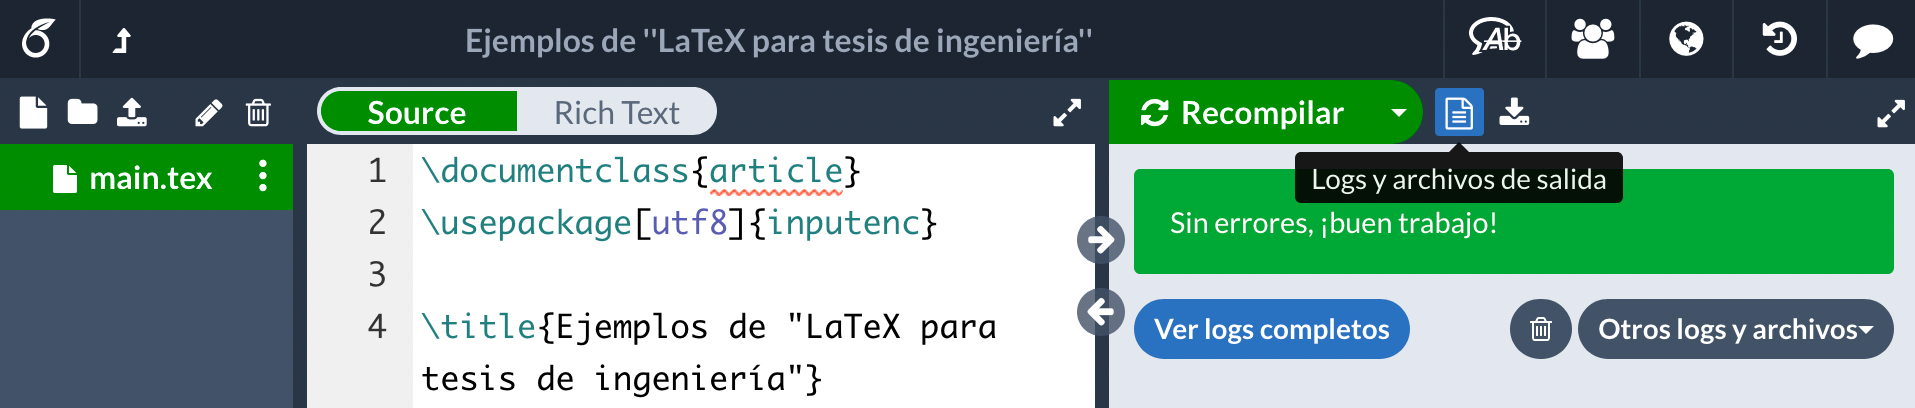
\includegraphics[width=\linewidth]{img/overleaf_boton_log_300ppi.png}
	\caption{Botón de \opcionMenu{Logs y archivos de salida} en Overleaf.}
	\label{fig:overleaf_boton_log}
\end{figure}

Al dar clic sobre dicho botón se abrirá un pequeño menú, como se muestra en la figura \ref{fig:overleaf_boton_cache}, que nos da acceso al botón \opcionMenu{Borrar archivos en la caché}, con el ícono de un bote de basura, que nos permite deshacernos de los archivos temporales asociados al proceso de compilación de nuestro proyecto o archivo.

\begin{figure}[ht!]
	\centering
	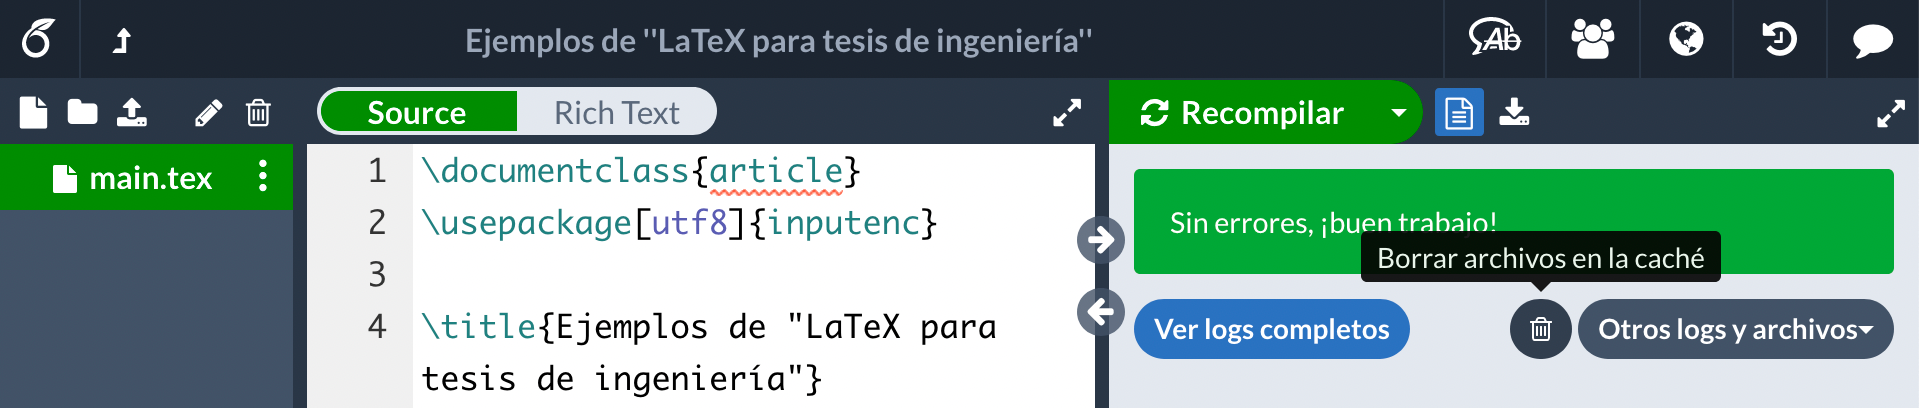
\includegraphics[width=\linewidth]{img/overleaf_boton_cache_300ppi.png}
	\caption{Botón de \opcionMenu{Borrar archivos en la caché} en Overleaf.}
	\label{fig:overleaf_boton_cache}
\end{figure}



\newpage
\section*{Resumen}



En este capítulo definimos qué es \LaTeX{} de una manera que facilita su interacción con el sistema e indagamos empíricamente qué hace cada línea del primer documento generado en la plataforma en línea Overleaf.

Además, establecimos dos consejos que te ayudarán mucho en tu aventura de terminar tu tesis con \LaTeX{}: compila frecuentemente y elimina archivos temporales después de una compilación fallida.

Armados con este conocimiento, estamos listos para empezar a ver cómo usar negritas, cursivas, y otras cosas de formato en \LaTeX{}.